\documentclass[border=2pt]{standalone}
\usepackage{fontspec}
\usepackage{unicode-math}
\setmainfont{Libertinus Serif}
\setsansfont{Libertinus Sans}
\setmathfont{Libertinus Math}[Scale=MatchUppercase]
\setmonofont{JetBrainsMono-Regular.ttf}[Path=../fonts/,ItalicFont=JetBrainsMono-Italic.ttf,Scale=0.95,RawFeature={-liga,-calt,-clig,-dlig}]
\usepackage{amsmath}
\providecommand{\llbracket}{[\![}
\providecommand{\rrbracket}{]\!]}
\usepackage{tikz}
\usetikzlibrary{positioning,arrows.meta,fit,backgrounds,calc,decorations.pathreplacing,decorations.markings,shapes.misc,matrix,shadings}

\definecolor{ink}{HTML}{1F2328}
\definecolor{muted}{HTML}{5B6470}
\definecolor{hairline}{HTML}{C9CFD6}
\definecolor{paper}{HTML}{FFFFFF}
\definecolor{pass}{HTML}{007A59}   \definecolor{passsoft}{HTML}{DAF1E9}
\definecolor{back}{HTML}{7A3E65}   \definecolor{backsoft}{HTML}{F1E1EB}
\definecolor{backdeep}{HTML}{70355C}
\definecolor{keep}{HTML}{006A91}   \definecolor{keepsoft}{HTML}{DCE9F5}
\definecolor{meas}{HTML}{9A5B00}   \definecolor{meassoft}{HTML}{FBEFD5}
\definecolor{measdeep}{HTML}{885000}
\definecolor{bad}{HTML}{AF4900}    \definecolor{badsoft}{HTML}{F9E1D3}
\definecolor{light}{HTML}{167BB4}  \definecolor{lightsoft}{HTML}{E3F2FB}

\tikzset{
  house/.style={>={Stealth[length=1.35mm, width=.95mm]}, line width=0.6pt,
    every node/.style={font=\small, text=ink}},
  flowmark/.style={postaction={decorate},decoration={markings,
    mark=at position .60 with {\arrow{Stealth[length=1.15mm,width=.8mm]}}}},
  box/.style={draw=ink, line width=0.6pt, rounded corners=1.8pt, inner xsep=5pt, inner ysep=3.5pt,
    align=center, fill=paper},
  boxdim/.style={box, draw=hairline, text=muted},
  boxpass/.style={box, draw=pass, shade,left color=passsoft!45!white,right color=passsoft},
  boxback/.style={box, draw=back, shade,left color=backsoft!45!white,right color=backsoft},
  boxkeep/.style={box, draw=keep, shade,left color=keepsoft!45!white,right color=keepsoft},
  boxmeas/.style={box, draw=meas, shade,left color=meassoft!45!white,right color=meassoft},
  boxbad/.style={box, draw=bad, shade,left color=badsoft!45!white,right color=badsoft},
  body/.style={box, shade,top color=white,bottom color=ink!5!white,
    minimum width=10mm, minimum height=11mm, font=\normalsize},
  wire/.style={draw=ink, line width=0.8pt},
  wpass/.style={draw=pass, line width=0.9pt},
  wback/.style={draw=back, line width=0.9pt},
  wkeep/.style={draw=keep, line width=0.9pt},
  wmeas/.style={draw=meas, line width=0.9pt},
  cwire/.style={draw=ink, line width=0.4pt, double, double distance=1.1pt},
  cmeas/.style={draw=meas, line width=0.45pt, double, double distance=1.1pt},
  flow/.style={->, draw=ink, line width=0.6pt},
  flowdim/.style={->, draw=muted, line width=0.5pt},
  lab/.style={font=\footnotesize, text=ink, inner sep=1.5pt},
  labpass/.style={lab, text=pass!80!black},
  labback/.style={lab, text=backdeep},
  labkeep/.style={lab, text=keep},
  labmeas/.style={lab, text=measdeep},
  labbad/.style={lab, text=bad},
  note/.style={font=\footnotesize, text=muted, align=left, inner sep=1.5pt},
  head/.style={font=\small\bfseries, text=ink, inner sep=1.5pt},
  panel/.style={font=\footnotesize\itshape, text=muted, inner sep=1.5pt},
  group/.style={draw=hairline, dashed, rounded corners=2.5pt, inner sep=5pt},
  gate/.style={draw=ink, fill=paper, line width=0.6pt, rounded corners=1.2pt, minimum size=6mm, inner sep=2pt},
  ctrl/.style={circle, fill=ink, inner sep=0pt, minimum size=1.6mm},
  octrl/.style={circle, draw=ink, fill=paper, inner sep=0pt, minimum size=1.6mm, line width=0.6pt},
  dot/.style={circle, fill=ink, inner sep=0pt, minimum size=1.5mm},
  meter/.style={draw=meas, fill=meassoft, line width=0.6pt, rounded corners=1.2pt, minimum width=7mm,
    minimum height=5.6mm, inner sep=0pt,
    path picture={\draw[measdeep, line width=0.5pt] ($(path picture bounding box.center)+(-2mm,-1.2mm)$) arc (180:0:2mm);
                  \draw[measdeep, line width=0.5pt, ->] ($(path picture bounding box.center)+(0,-1.2mm)$) -- ++(1.4mm,2.1mm);}},
  cell/.style={draw=hairline, minimum width=7mm, minimum height=5.5mm, inner sep=0pt, font=\footnotesize},
}
\newcommand{\feedbackcurve}[3]{\draw[wback, postaction={decorate}, decoration={markings, mark=at position .5 with {\arrow{Stealth[length=1.3mm,width=.9mm]}}}]
    ($(#1.east)+(0,-2.6mm)$) -- ($(#1.east)+({max(#3-0.55,0.15)},-2.6mm)$)
    to[out=0,in=0,looseness=1.7] ($(#1.east)+({max(#3-0.55,0.15)},-2.6mm)+(0,-#2)$)
    -- ($(#1.west)+({-max(#3-0.55,0.15)},-2.6mm)+(0,-#2)$)
    to[out=180,in=180,looseness=1.7] ($(#1.west)+({-max(#3-0.55,0.15)},-2.6mm)$)
    -- ($(#1.west)+(0,-2.6mm)$);}
\newcommand{\feedbackcurvez}[4]{\draw[wback]
    ($(#1.east)+(0,-2.6mm)$) -- ($(#1.east)+({max(#3-0.55,0.15)},-2.6mm)$)
    to[out=0,in=0,looseness=1.7] ($(#1.east)+({max(#3-0.55,0.15)},-2.6mm)+(0,-#2)$)
    -- node[boxback, font=\footnotesize, inner xsep=3pt, inner ysep=2pt] {#4}
       ($(#1.west)+({-max(#3-0.55,0.15)},-2.6mm)+(0,-#2)$)
    to[out=180,in=180,looseness=1.7] ($(#1.west)+({-max(#3-0.55,0.15)},-2.6mm)$)
    -- ($(#1.west)+(0,-2.6mm)$);
  \draw[wback,-{Stealth[length=1.3mm,width=.9mm]}] ($(#1.west)+(-0.12,-2.6mm)+(0,-#2)$) -- ++(-0.01,0);}
\newcommand{\feedbackcurveat}[4]{\draw[wback, postaction={decorate}, decoration={markings, mark=at position .5 with {\arrow{Stealth[length=1.3mm,width=.9mm]}}}]
    ($(#1.east)+(0,-#2)$) -- ($(#1.east)+({max(#4-0.55,0.15)},-#2)$)
    to[out=0,in=0,looseness=1.7] ($(#1.east)+({max(#4-0.55,0.15)},-#2)+(0,-#3)$)
    -- ($(#1.west)+({-max(#4-0.55,0.15)},-#2)+(0,-#3)$)
    to[out=180,in=180,looseness=1.7] ($(#1.west)+({-max(#4-0.55,0.15)},-#2)$)
    -- ($(#1.west)+(0,-#2)$);}
\newcommand{\backloop}[3]{\draw[wback, rounded corners=3pt] ($(#1.east)+(0,-2.6mm)$) -- ++(#3,0) -- ++(0,-#2) -- ($(#1.west)+(-#3,-2.6mm)+(0,-#2)$) -- ($(#1.west)+(-#3,-2.6mm)$) -- ($(#1.west)+(0,-2.6mm)$);}
\newcommand{\ket}[1]{\lvert #1\rangle}
\newcommand{\bra}[1]{\langle #1\rvert}
\newcommand{\kw}[1]{\texttt{#1}}
\providecommand{\Tr}{\operatorname{Tr}}
\hyphenpenalty=10000 \exhyphenpenalty=10000

\begin{document}
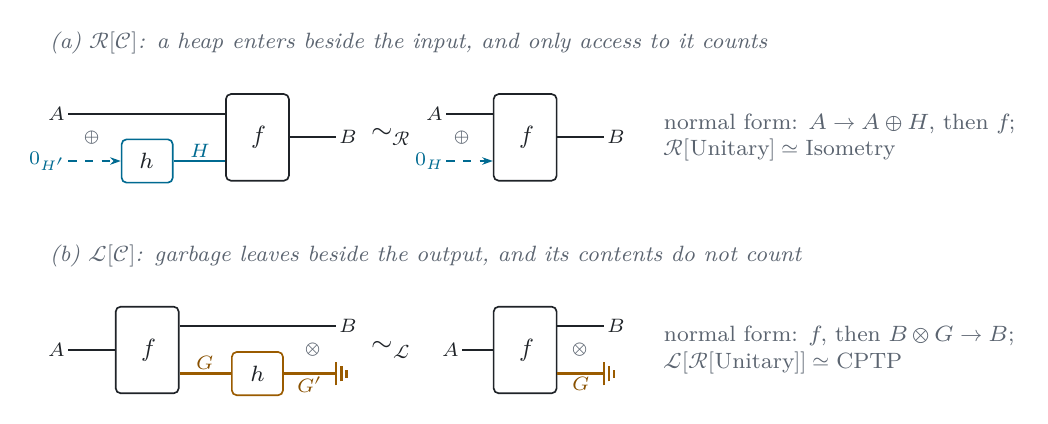
\begin{tikzpicture}[house, x=1mm, y=1mm,
  op/.style={box, minimum width=8mm, minimum height=11mm, inner sep=1pt, font=\small},
  sm/.style={box, minimum width=6.5mm, minimum height=5.5mm, inner sep=1pt, font=\footnotesize},
  wl/.style={font=\scriptsize, inner sep=0.8pt},
  eq/.style={font=\normalsize}]
\node[panel, anchor=west] at (-3,12) {(a) $\mathcal R[\mathcal C]$: a heap enters beside the input, and only access to it counts};
\node[sm, draw=keep] (h) at (10,-3) {$h$};
\node[op] (f) at (24,0) {$f$};
\draw[wire] (0,3) node[wl, left] {$A$} -- (f.west |- 0,3);
\draw[wkeep,dashed,->] (0,-3) node[wl, left, text=keep] {$0_{H'}$} -- (h.west);
\draw[wkeep] (h.east) -- node[wl, above, text=keep] {$H$} (f.west |- 0,-3);
\draw[wire] (f.east) -- (34,0) node[wl, right] {$B$};
\foreach \x in {3,50} \node[wl,text=muted] at (\x,0) {$\oplus$};
\node[eq] at (41,0) {$\sim_{\mathcal R}$};
\node[op] (f2) at (58,0) {$f$};
\draw[wire] (48,3) node[wl, left] {$A$} -- (f2.west |- 0,3);
\draw[wkeep,dashed,->] (48,-3) node[wl, left, text=keep] {$0_H$} -- (f2.west |- 0,-3);
\draw[wire] (f2.east) -- (68,0) node[wl, right] {$B$};
\node[note, anchor=west, align=left] at (75,0) {normal form: $A\to A\oplus H$, then $f$;\\ $\mathcal R[\mathrm{Unitary}]\simeq\mathrm{Isometry}$};
\begin{scope}[yshift=-27mm]
\node[panel, anchor=west] at (-3,12) {(b) $\mathcal L[\mathcal C]$: garbage leaves beside the output, and its contents do not count};
\node[op] (g) at (10,0) {$f$};
\node[sm, draw=meas] (k) at (24,-3) {$h$};
\draw[wire] (0,0) node[wl, left] {$A$} -- (g.west);
\draw[wire] (g.east |- 0,3) -- (34,3) node[wl, right] {$B$};
\draw[wmeas] (g.east |- 0,-3) -- node[wl, above, text=measdeep] {$G$} (k.west);
\draw[wmeas] (k.east) -- node[wl,below,text=measdeep] {$G'$} (34,-3);
\foreach \x in {31,65} \node[wl,text=muted] at (\x,0) {$\otimes$};
\node[eq] at (41,0) {$\sim_{\mathcal L}$};
\node[op] (g2) at (58,0) {$f$};
\draw[wire] (50,0) node[wl, left] {$A$} -- (g2.west);
\draw[wire] (g2.east |- 0,3) -- (68,3) node[wl, right] {$B$};
\draw[wmeas] (g2.east |- 0,-3) -- node[wl,below,text=measdeep] {$G$} (68,-3);
\foreach \x in {34,68} {
  \draw[wmeas] (\x,-4.5) -- (\x,-1.5)
    (\x+.65,-4.0) -- (\x+.65,-2.0) (\x+1.3,-3.5) -- (\x+1.3,-2.5);
}
\node[note, anchor=west, align=left] at (75,0) {normal form: $f$, then $B\otimes G\to B$;\\ $\mathcal L[\mathcal R[\mathrm{Unitary}]]\simeq\mathrm{CPTP}$};
\end{scope}
\end{tikzpicture}
\end{document}
